\documentclass[a4paper]{article}


\usepackage[student]{Lecture-TD}

\lhead{Travaux dirigés - Structure $\oplus$}% des accumulateurs
\lfoot{IUT d'Orsay - BUT 2A - 2024/2025} \cfoot{
\includegraphics[height=0.5cm]{cc-by-nc-sa.png}}  \rfoot{Jean-François Olivieri \quad \thepage}

\begin{document}

\begin{center}
\begin{minipage}{0.7\textwidth}
\centering
\Large \textbf{TD n$^\circ ~ 4$} \\
Structure des matériaux d'insertion du pôle $\oplus$
\end{minipage}
\end{center}

\objectives{
\begin{itemize}
\item Connaître les principales caractéristiques cristallographiques des structures lamellaires, des spinelles et des olivines ;
\item Interpréter ou établir la dimension du matériau ;
\item Interpréter la connectivité des polyèdres de coordination ;
\item Justifier la capacité d'un matériau à accueillir du lithium et interpréter, dans le cadre de liaisons supposées ioniques, la stabilité éventuelle de ces sites par des considérations : stériques \& énergétique (modèle du champ cristallin) ;
\item Savoir rendre compte de l'effet de la déformation d'un polyèdre de coordination  sur la position des orbitales $d$ du métal : exemple de l'effet Jahn-Teller dans les spinelles.
\end{itemize}
}

\cteacher{Dans ce TD, on va chercher à donner une interprétation microscopique à la stabilité des matériaux dans le cas de la lithiation ou de la délithiation d'un matériau par le lithium. Ce TD réutilise des concepts vus en BUT1 et BUT2 : atomistique, champ cristallin et cristallographie pour donner des considérations énergétiques aux observations structurales, que l'on peut faire, des matériaux lithiés à un état de charge donné. \\
Vous pouvez traiter uniquement la première partie sur les matériaux lamellaires dans ce TD. Si vous êtes juste en temps, vous pouvez sauter l'exercice \ref{subsubsection:oxyde_lamellaire} en résumant juste les principales conclusions et mettre l'accent sur l'exercice \ref{subsection:iono-covalent-bond}.
\emph{NB} Sur la structure \ce{LiCoO2}, les exercices traitent cette maille comme hexagonale, ce qui n'est pas tout à fait vrai. Je n'ai pas corrigé cette erreur pour cette année par souci de simplicité pour les étudiants... en mon sens, ce n'est pas critique.
}

\section{Structures lamellaires}

\subsection{L’oxyde lamellaire : reférence \ce{LiCoO2}}
\label{subsubsection:oxyde_lamellaire}

\setcounter{equation}{0}
\setcounter{Q}{0}

\begin{center}
\begin{minipage}[]{0.2\textwidth}
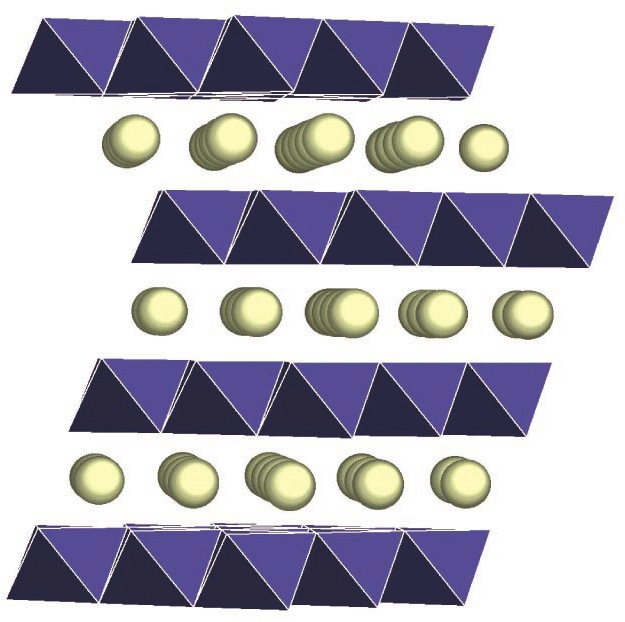
\includegraphics[height=3cm]{Ex16/Fig01c}
\end{minipage}\begin{minipage}[]{0.3\textwidth}
\captionof{figure}{Représentation de la structure sous forme de polyèdre}
\label{fig:Ex16-Fig02}
\end{minipage}
\end{center}

Comme représenté à la Fig. \ref{fig:Ex16-Fig02}, les composés lamellaires résultent d'un empilement successif :
\begin{enumerate}
\item d'octaèdres \ce{MO6}, où M est le métal participant à la "charpente" de la couche d'oxyde ;
\item d'une couche de lithium occupant des sites octaédriques, tétraédriques ou prismatiques.
\end{enumerate}

Nous allons chercher à comprendre comment visualiser ces structures en partant de vos notions élémentaires en cristallographie. Une façon de voir ces structures est de considérer une maille élémentaire où :
\begin{enumerate}
\item les métaux Li ou M occupent un réseau cubique à face centré ;
\item les oxygènes occupent tous les sites octaédriques de ce réseau.
\end{enumerate}

%Review—Li-Rich Layered Oxide Cathodes for Next-Generation Li-Ion Batteries: Chances and Challenges

\Q \label{Q:Ex16-1} Représenter la maille élémentaire CFC ainsi que les sites occupés. Indiquer le repère $(\vec{a}_c, \vec{b}_c, \vec{c}_c)$ dans ce système cubique.
\solution{Représentation du système cubique face centré en question :
\begin{center}

\includegraphics[width=0.48\textwidth]{Ex16/Corr01}
\end{center}
Les atomes d'oxygènes (resp. atomes métalliques) sont indiqués en rouge (resp. gris)
}

\Q \label{Q:Ex16-2} Identifier un axe de plans réticulaires de la maille cubique permettant de rendre compte de l'aspect lamellaire de la structure. Nommer cette série de plans.
\solution{On remarque qu'en prenant l'axe réticulaire [111], on obtient bien une succession de plans d'oxygène et de cation : 
\begin{center}

\includegraphics[width=0.35\textwidth]{Ex16/Corr02}
\end{center}
}

\Q Afin d'aboutir à une structure lamellaire à partir de la structure cubique, une projection a été proposée selon le plan définit par les vecteurs de base :

\begin{minipage}{0.48\textwidth}
\begin{align*}
\left(  \frac{\vec{a}_c + \vec{b}_c}{2} , \vec{c}_c \right)
\end{align*}
\end{minipage}\hfill \begin{minipage}{0.48\textwidth}

\includegraphics[width=\textwidth]{Ex16/Fig02}
\end{minipage}

La maille élementaire a volontairement été multipliée par 4 selon les trois axes unitaires du cube (c.-à-d. que le volume de la maille a été multiplié $\times 4^3 = 32$) . Identifier les centres métalliques qui doivent être des \ce{Li} et ceux qui doivent être des \ce{Co}. Représenter la maille élémentaire hexagonale résultante.
\solution{Un plan sur deux de cations contient des cations de lithium (gris) et l'autre des cations de cobalt (bleu).
\begin{center}
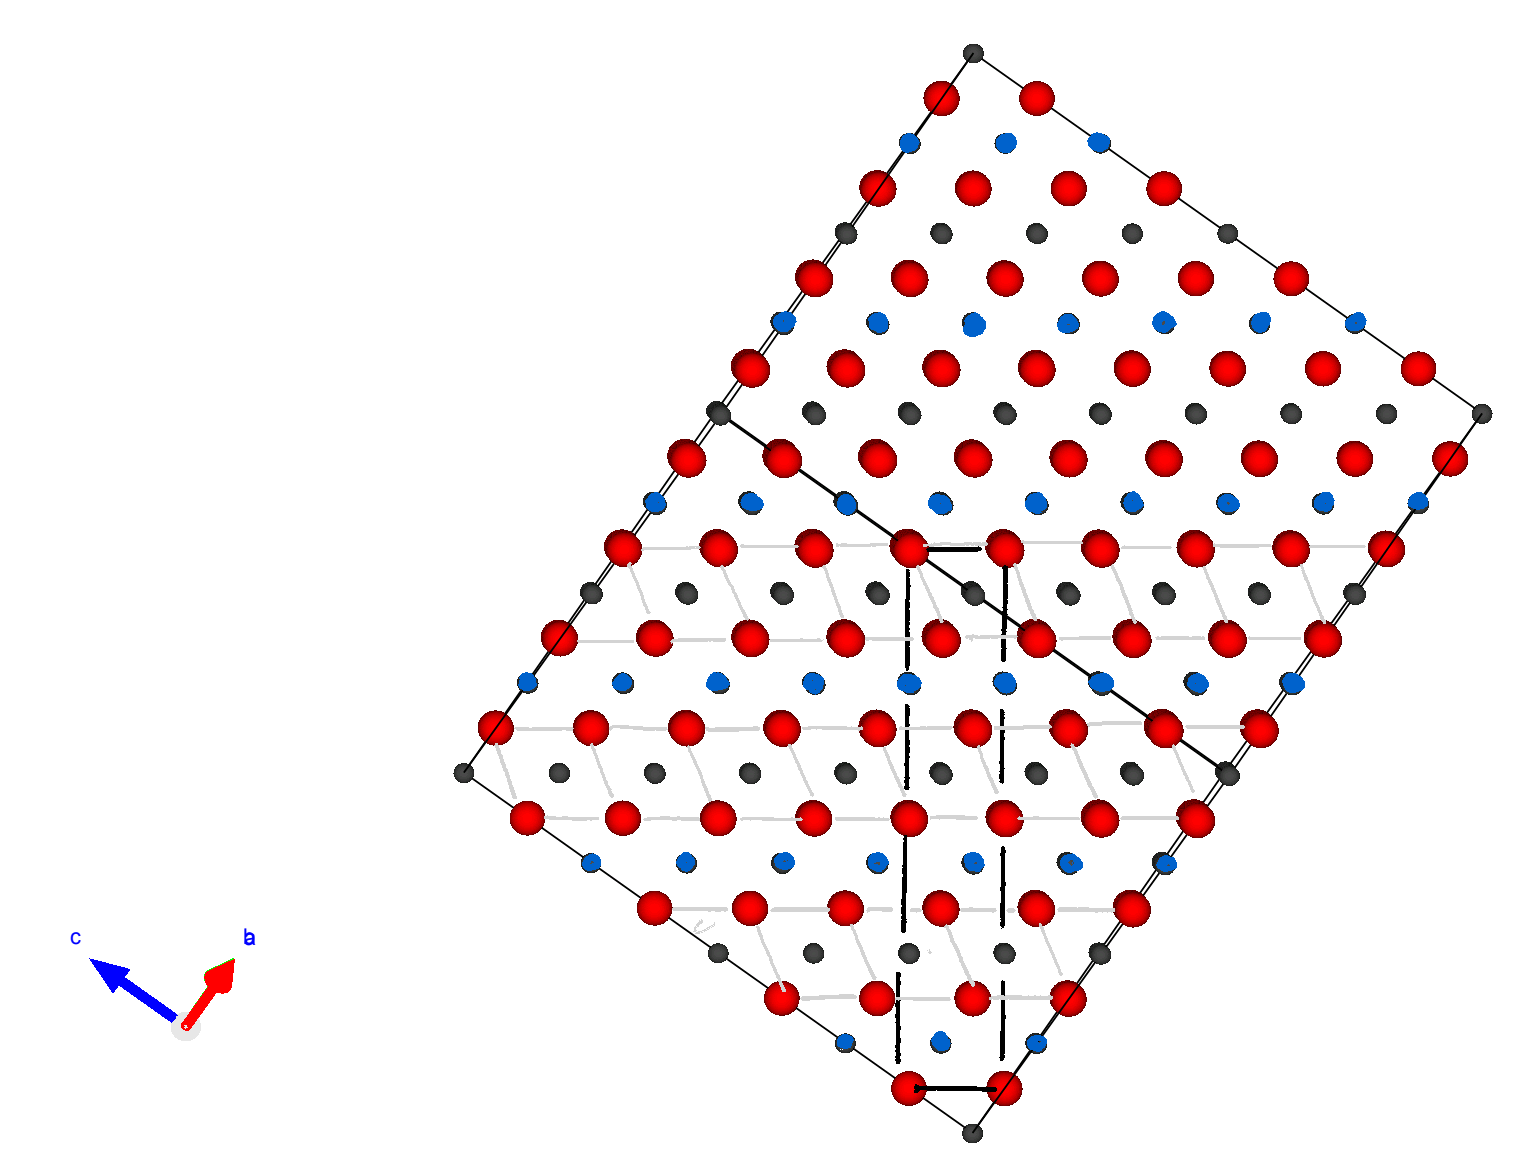
\includegraphics[width=0.35\textwidth]{Ex16/Corr03}
\end{center}
On représente la plus petite maille hexagonale résultante.
}

\begin{comment}
\Q Définir un nouveau repère $(\vec{a}_h, \vec{b}_h, \vec{c}_h)$ à partir des vecteurs de base de la Q.\ref{Q:Ex16-1}. Renommer le plan réticulaire trouvé à la Q.\ref{Q:Ex16-2} dans le système hexagonal.
\solution{
\begin{align*}
\vec{a}_h &= \\
\vec{b}_h &= \\
\vec{c}_h &= \frac{1}{\sqrt{3}}(\vec{a}_c + \vec{a}_c + \vec{a}_c)
\end{align*}
}\end{comment}


Après toutes ces constructions, la maille obtenue pour l'oxyde lamellaire \ce{LiCoO2}, matériau de la première batterie Sony (1990). Sa structure est projetée aux Fig.\ref{fig:Ex16-01a} et \ref{fig:Ex16-01b} selon les plans réticulaires (100) et (001) définis dans le nouveau repère hexagonal.

\begin{center}
\begin{minipage}[]{0.4\textwidth}
\begin{figure}[H]
\begin{centering}
\subfloat[\label{fig:Ex16-01a}]{
\includegraphics[width=2cm]{Ex16/Fig01a}}\hfill
\subfloat[\label{fig:Ex16-01b}]{
\includegraphics[height=3cm]{Ex16/Fig01b}}
\end{centering}
\end{figure}
\end{minipage}\hspace{0.5cm}\begin{minipage}[]{0.4\textwidth}
\captionof{figure}{\ref{fig:Ex16-01a} Maille conventionnelle du composé de st{\oe}chiométrie \ce{Li3Co3O6} projetée le long de (100). \ref{fig:Ex16-01b} Maille conventionnelle du composé de st{\oe}chiométrie \ce{Li3Co3O6} projetée le long de (001).}
\end{minipage}
\end{center}

\Q Nommer cette structure dans la nomenclature de Delmas. Justifier si l'interaction Li-O est plutôt de nature ionique ou covalente.
\solution{
Les atomes de lithium sont liés aux oxygènes par des octaèdres, on qualifie la structure de O. Il y a 3 plaques d'oxyde de cobalt dans la maille, on peut donc dire que la structure est \ce{O3}. Au bilan, cette variété allotropique de l'oxyde de cobalt lithié est qualifié par : 
\begin{align*}
\ce{O3-LiCoO3}
\end{align*}
\`{A} partir des données, on peut calculer la distance Li-O et calculer l'écart à l'expérience : 
\begin{center}
\begin{tabular}{ccc}
\toprule
Type de liaison & Longueur de liaison & \'{E}cart relatif \\
& \si{\pico\meter} & $\emptyset$ \\
\midrule
covalente & $134 + 66 = 200$ & $\frac{209-200}{209} \approx 0.04$\\
ionique & $128 + 76 = 204$ & $\frac{209-204}{209} \approx 0.02$\\
\bottomrule
\end{tabular}
\end{center}
où l'écart relatif est calculé comme : 
\begin{align*}
\frac{d_{Li-O}^{calc} - d_{Li-O}^{exp}}{d_{Li-O}^{exp}}
\end{align*}
De plus, en calculant de degré d'ionicité à l'aide du modèle de Pauling, on trouve : 
\begin{align*}
I = 0.78 = 78 ~ \si{\percent}
\end{align*}
\`{A} priori, ces deux arguments (surtout le second) sont en faveur d'une liaison plutôt ionique.}%O3-LiCoO3

Une autre façon de représenter la maille est d'ajouter les polyèdres de coordinations au sein de la maille. La structure cristallographique est représentée en perspective sur la Fig. \ref{fig:16-04}.

\begin{center}
\begin{minipage}[]{0.4\textwidth}
\begin{figure}[H]
\begin{centering}

\includegraphics[width=3cm]{Ex16/Fig04}
\end{centering}
\end{figure}
\end{minipage}\hspace{0.5cm}\begin{minipage}[]{0.4\textwidth}
\captionof{figure}{Polyèdres de coordination du lithium et du cobalt sur une représentation en perspective de la maille du composé de st{\oe}chiométrie \ce{Li3Co3O6}.}
\label{fig:16-04}
\end{minipage}
\end{center}


\Q Indiquer comment les octaèdres sont coordonnés entre eux.
\solution{
On a deux types d'octaèdres : \ce{CoO6} et \ce{LiO6}. Il y a donc trois coordinations possibles entre les octaèdres : 
\begin{center}
\begin{tabular}{ccc}
\hline
\ce{LiO6}-\ce{LiO6} & \ce{LiO6}-\ce{CoO6} & \ce{CoO6}-\ce{CoO6} \\
\hline
arêtes & arêtes & arêtes \\
\hline
\end{tabular}
\end{center}
}

\Q Quelle est la charge électrique des feuillets composés de polyèdres cobalt-oxygène ? 
\solution{Les ions lithium entre les feuillets sont chargés positivement. Par électroneutralité de la structure, les feuillets sont donc chargés négativement.}

\Q Cette première batterie possédait une capacité spécifique de \SI{150}{\milli\ampere\hour\per\gram} ce qui est relativement faible (on peut maintenant obtenir le double). Proposer une hypothèse expliquant cette capacité relativement faible.
\solution{Les feuillets sont chargés négativement. Une partie des ions lithium doivent nécessairement rester entre les plaques pour stabiliser la structure. Par conséquent, lors d'une charge, tous les ions lithium ne peuvent pas quitter la structure.}

\Q Comment peut-on améliorer la situation ? Pourquoi ? 
\solution{On doit stabiliser la structure cristallographique en :
\begin{itemize}
\item utilisant des cations de plus haut degré d'oxydation ; 
\item utilisant des anions plus polarisables (gros).
\end{itemize}
}

Quelques-unes de ces améliorations de la structure \ce{LiCoO2} sont étudiées en détails dans le dernier chapitre du cours.

\paragraph*{Données}
\begin{itemize}
\item Distance expérimentale \ce{Li-O} dans \ce{LiCoO2} : $d^{exp}_{Li-O} = 209 ~ \si{\pico\meter}$   
\item Rayons ioniques en \si{\pico\meter} : 
\begin{align*}
r_{Li} ( \text{IV} ) &= 59 ~ \si{\pico\meter} ; \\
r_{Li} ( \text{VI} ) &= 76 ~ \si{\pico\meter} ; \\
r_{O} &= 128 ~ \si{\pico\meter} ;
\end{align*}
\item Rayons covalents en \si{\pico\meter} : 
\begin{align*}
r_{Li} &= 134 ~ \si{\pico\meter} ; \\
r_{O} &= 66 ~ \si{\pico\meter}
\end{align*}
\item \'{E}lectronégativité de Pauling : 
\begin{align*}
\chi ( \ce{Li} ) &= 0.98 \\
\chi ( \ce{O} ) &= 3.44 \\
\end{align*}
\item Pauling est le premier à avoir défini le degré d'ionicité et a montré que dans nombre de composés ioniques \ce{A}-\ce{B}, l'ionicité de la liaison est "bien décrite" par la relation suivante : 
\begin{align*}
I = 1 - \exp \left( - \frac{( \chi (\ce{A}) - \chi (\ce{B}))^2}{4} \right)
\end{align*}
où $\chi$ est l'électronégativité du composé $A$ ou $B$ dans l'échelle de Pauling.
\end{itemize}


\subsection{Liaison iono-covalente}
\label{subsection:iono-covalent-bond}


\setcounter{equation}{0}
\setcounter{Q}{0}

Le dioxyde de cobalt \ce{Li_xCoO2} est étudié à l'aide d'une courbe de charge/décharge à une vitesse $C/24$ sur une plage de potentiel de $3.6$ à \SI{4.85}{\volt/{Li^+ / Li}}. La courbe de charge/décharge suivante est obtenue :

\begin{center}
\begin{minipage}[]{0.6\textwidth}
\centering

\includegraphics[height=5cm]{Ex18/Fig01}
\end{minipage}\begin{minipage}[]{0.3\textwidth}
\captionof{figure}{Courbes de charge/décharge de \ce{Li_xCoO2} à un courant électrique valant $C/24$.}
\label{fig:18-01}
\end{minipage}
\end{center}

La capacité spécifique expérimentale de la cathode vaut : $C = 140 ~ \si{\milli\ampere\hour\per\gram}$. Il est courant d'exprimer le courant en l'indiquant sous la forme :
\begin{align*}
\text{courant (massique)} = \frac{\text{capacité (spécifique massique) de la cellule}}{\text{durée de la décharge}}
\end{align*}

\Q Quel est le sens du terme $C/24$ ? Trouver le courant appliqué par gramme de matériau.

\solution{
Le courant $C/24$ signifie que l'on a déchargé le matériau à vitesse constante de telle sorte que la batterie atteigne l'état $SoC=0 ~ \si{\percent}$ en \SI{24}{\hour}. Par conséquent, la vitesse par gramme de matériau, notée $I_m$, vaut : 
\begin{align*}
I_m = \frac{C}{\Delta t} \stackrel{AN}{=} \frac{140}{24} \approx 5.8 ~ \si{\milli\ampere\per\gram}. 
\end{align*}
\faWarning ~ Cette notation n'est pas abordée dans le cours. Elle est précisée dans cet exercice, question de dire qu'elle ne soit pas étrangère aux étudiants si elle est rencontrée dans une publication. On trouve des tonnes de discussion en ligne sur cette notation, ils n'auront aucun soucis à se débrouiller avec si elle est rencontrée. En partiel, la définition de la notation sera donnée dans les données si nécessaire.
}

\Q Donner l'évolution des degrés d'oxydation de l'oxygène et du cobalt lors de la charge dans un modèle de liaison \SI{100}{\percent} ionique.
\solution{En utilisant l'équation de conservation de la charge dans un composé $\ce{Li_x Co O2}$: 
\begin{align*}
x \cdot no (\ce{Li}) + no (\ce{Co}) + 2 \cdot no (\ce{O}) = 0
\end{align*}
On en déduit les résultats suivants pour les motifs limites : 
\begin{center}
\begin{tabular}{ccc}
\toprule
SoC & \SI{0}{\percent} & \SI{100}{\percent} \\
Fraction lithium x & 1 & 0 \\
\midrule
$no (\ce{Co})$ & $+III$ & $+IV$ \\
$no (\ce{O})$ & $-II$ & $-II$ \\
\bottomrule
\end{tabular}
\end{center}
}

On rappelle que la structure de \ce{LiCoO2} est lamellaire et que cette structure est décrite par une maille hexagonale. La structure lithiée a été suivie par DRX. On a constaté que pour $x > 0.5$, la structure ne subit aucun changement dans ses paramètres de maille. Cependant, pour $x<0.5$, on constate que le rapport $c/a$ de la maille hexagonale diminue.

\Q En vous appuyant sur la structure lamellaire, que peut traduire microscopiquement une diminution du rapport $c/a$ ?
\solution{Une diminution du rapport $c/a$ traduit le fait que l'espace entre les plaques diminue. Or, on sait que l'origine de la distance entre les plaques est électrostatique : c'est la répulsion entre les charges partielles négatives des oxygènes qui se font face.}

On a vu que le cobalt est entouré d'oxygène dans un environnement octaédrique, de coordinence [6]. 

\Q En vous appuyant sur le modèle du champ cristallin, rappeler, en le justifiant, le diagramme d'orbitale du bloc $d$ du cobalt $+III$.

Il a été expérimentalement observé que lors du passage de $x = 1$ à $x = 0$, une transition de spin, d'une structure bas spin à une structure haut spin. La mesure expérimentale de l'évolution des longueurs de liaison a montré que selon la direction $z$, il y a un allongement significatif des octaèdres de cobalt conjointe à une compression dans la direction $xy$.

\Q Cette observation est-elle en accord avec les mesures de DRX précédente ?

\solution{La structure DRX nous donne un allongement selon la direction $c$ et une compression selon la direction $a$. Cette observation est en accord avec les mesures réalisées sur les longueurs de liaisons.}


\Q \`{A} partir du diagramme d'énergie de l'octaèdre prédit par le champ cristallin, proposer une structure électronique qui rende compte du nouvel état de spin.

\emph{NB : On va supposer que la déformation est suffisante pour que le niveau $d z^2$ devienne plus stable que le niveau $d_{x^2 - y^2}$}

\solution{
En cas d'expansion de l'octaèdre dans la direction $z$ et une contraction dans la direction $xy$, on s'attend à une :
\begin{itemize}
\item diminution de la répulsion entre les électrons du métal et des ligands dans la direction $z$, donc une forte stabilisation en énergie de la $d_{z^2}$ et dans une moindre mesure des $d_{xz} $ et $d_{yz}$ ;
\item augmentation de la répulsion dans le plan $xy$ entre les électrons du métal et des ligands, donc une forte déstabilisation en énergie de la $d_{x^2 - y^2}$ et dans une moindre mesure de la $d_{xy}$.
\end{itemize}
\begin{center}
\begin{minipage}{0.5\textwidth}

\includegraphics[width=\textwidth]{Ex39/Fig03a}
\end{minipage}\begin{minipage}{0.46\textwidth}
orbitales {\color{red} -} destabilisées \\
orbitales {\color{blue} -} stabilisées
\end{minipage}
\end{center}
L'octaèdre déformé correspond à la structure délithié $\ce{CoO2}$ et l'octaèdre parfait à la structure lithié \ce{LiCoO2}. Par conséquent, on s'attend à avoir une structure $d^6$ champ fort, bas spin pour l'octaèdre parfait, et une structure $d^5$ pour l'octaèdre déformé.
\begin{center}

\includegraphics[width=0.5\textwidth]{Ex39/Fig03b}
\end{center}
}


\Q En vous appuyant sur une interaction selon l'axe $z$ entre une orbitale $d_{z^2}$ et une orbitale $2p_z$, montrer la différence entre l'oxydation dans un modèle purement ionique et un modèle iono-covalent.
\solution{
Dans un modèle ionique, l'écart en énergie des orbitales est suffisamment grand pour que les orbitales du métal soient les seules à perdre des électrons : 
\begin{center}
\begin{minipage}{0.48\textwidth}
\centering

\includegraphics[width=\textwidth]{Ex39/Fig01a}
Avant oxydation
\end{minipage}\hfill \begin{minipage}{0.48\textwidth}
\centering

\includegraphics[width=\textwidth]{Ex39/Fig01b}
Après oxydation
\end{minipage}
\end{center}
Dans un modèle iono-covalent, l'orbitale oxydée présente de la densité électronique sur le métal, mais aussi, dans une moindre mesure, sur l'oxygène :
\begin{center} 
\begin{minipage}{0.48\textwidth}
\centering

\includegraphics[width=\textwidth]{Ex39/Fig02a}
Avant oxydation
\end{minipage}\hfill \begin{minipage}{0.48\textwidth}
\centering

\includegraphics[width=\textwidth]{Ex39/Fig02b}
Après oxydation
\end{minipage}\end{center}}

\Q Que peut-on dire de l'évolution de la charge partielle aux oxygène dans un modèle ionocovalent ?

\solution{
Le diagramme d'interaction ionocovalent montre qu'après oxydation, les électrons occupant l'orbitale moléculaire antiliante  $d_{z^2} - p_z$ sont perdus. Puisqu'il y a de la densité électronique sur l'oxygène, c'est-à-dire que l'électron avait une probabilité non nul d'être sur l'oxygène, l'oxydation conduit à une diminution de la charge partielle portée par l'oxygène.
}



\section{Structures spinelles et olivines}

\subsubsection{Structure des matériaux de type spinelle (\ce{AB2X4})}

\setcounter{equation}{0}
\setcounter{Q}{0}

Certains spinelles peuvent être utilisés dans le domaine des batteries. En effet, ce type de matériaux présente une structure en 3D avec des canaux pouvant accueillir des ions lithium.

\`{A} l'état solide, l'oxyde de lithium-manganèse \ce{Li_x Mn_2 O_4} cristallise dans un réseau de type spinelle, comme présenté ci-dessous : 

\begin{center}

\includegraphics[width=10cm]{Ex12/Fig01}
\captionof{figure}{Projection 2D de la structure \ce{LiMn2O4} (a) et structure 3D (b)}
\end{center}


\Q Rappeler la différence entre spinelle normal et spinelle inverse.
\solution{Les spinelles présentent deux fois plus de sites tétraédriques (T) qu'octaédriques (O), on a donc deux occupations possibles des sites : 
\begin{align*}
\ce{[A]_O [B_2 ]_T O4} &\implies \text{spinelle inverse} \\
\ce{[B]_O [A B ]_T O4} &\implies \text{spinelle normal} \\
\end{align*}}

\Q \`{A} partir d'un calcul du degré d'oxydation, montrer que \ce{LiMn2O4} est un composé de valence mixte.
\solution{
Par électroneutralité, on a : 
\begin{align*}
no ( \ce{Li} ) + 2 \cdot no ( \ce{Mn} ) + 4 \cdot no ( \ce{O} ) = 0
\end{align*}
Avec les électronégativités, on a $\chi ( \ce{Li} ) < \chi ( \ce{Mn} ) < \chi ( \ce{O} )$, on a donc $no ( \ce{O} ) = - II$ et $no ( \ce{Li} ) = + I$ : 
\begin{align*}
2 no ( \ce{Mn} ) = VII \implies no( \ce{Mn}) = III \quad no ( \ce{Mn} ) = IV
\end{align*}
Les degrés d'oxydation stable du manganèse permettent de déterminer la seule solution.}

Dans une structure spinelle, les ions \ce{O^{2-}} occupent les n{\oe}uds d'un réseau cubique à faces centrées, les ions métalliques se répartissant entre les sites octaédriques et tétraédriques du réseau.

\Q Indiquer la position des sites octaédriques et tétraédriques dans le réseau cubique à faces centrées. Dénombrer ces sites. 
\solution{On va dénombrer le nombre de sites octaédrique et tétraédrique, la multiplicité vaut : 
\begin{align*}
Z ( \ce{O^{2-}} ) &= 8 \times \frac{1}{8} +  6 \times \frac{1}{2} = 4 \\
Z ( Td ) &= 8 \\
Z ( Oh ) &= 12 \times \frac{1}{4} + 1 = 4
\end{align*}}

Dans ces structures, les ions manganèse au degré d'oxydation III et IV occupent les sites octaédriques. Cependant, durant des cycles de charge/décharge rapides ou menées à trop grande tension, les ions manganèse migrent parfois dans des sites tétraédriques.

\Q En utilisant le \og critère stérique \fg{}, justifier pourquoi l'ion manganèse peut facilement migrer d'un site octaédrique vers un site tétraédrique.
\solution{On peut calculer le rapport entre le rayon de l'anion et du cation : 
\begin{align*}
r( \ce{Mn^{3+}}, \text{HS}) &= 65 ~ \si{\pico\meter} &\implies \rho_1 = 0.46\\
r( \ce{Mn^{3+}}, \text{BS}) &= 58 ~ \si{\pico\meter} &\implies \rho_2 = 0.41\\
r( \ce{Mn^{4+}} ) &= 53 ~ \si{\pico\meter} &\implies \rho_3 = 0.38
\end{align*}
Selon le \og critère stérique \fg{}, les cations manganèse IV et III-BS (resp. III-HS) occupent les sites tétraédriques (resp. octaédriques). Toutes ces valeurs sont "proches" de la valeur de transition Td-Oh.}

\Q Donner la configuration électronique des ions manganèse (III) et (IV).
\solution{
D'après les règles de l'Aufbau, on a : 
\begin{align*}
[\ce{Mn}] &= ~ _{18}[\ce{Ar}] 4s^2 3d^5 \\
[\ce{Mn^{3+}}] &= ~ _{18}[\ce{Ar}] 4s^0 3d^4 \\
[\ce{Mn^{4+}}] &= ~ _{18}[\ce{Ar}] 4s^0 3d^3 \\
\end{align*}
}

\Q En utilisant le \og critère énergétique \fg{}, justifier pourquoi l'ion manganèse (III) peut facilement migrer d'un site octaédrique vers un site tétraédrique. On présumera que sa configuration est haut-spin (HS) et on la précisera.
\solution{
La configuration électronique de Mn(III) HS est  : 
\begin{align*}
(t_{2g})^3 (e_g)^1
\end{align*}
On va chercher à estimer l'énergie de stabilisation du champ cristallin (ESCC) dans les trois configurations possibles du manganèse (III) : 
\begin{align*}
ESCC (Oh) &= - \frac{3}{5} \Delta_O \\ 
ESCC (Td) &= - \frac{2}{5} \Delta_T = - \frac{8}{45} \Delta_O
\end{align*}
On peut alors calculer la différence d'ESCC :
\begin{align*}
ESCC ( Oh, \text{HS} ) - ESCC (Td) &= -\frac{3}{5} \Delta_O  + \frac{8}{45} \Delta_O \\
&= - \frac{19}{45} \Delta_O \approx - 0.422 \Delta_O
\end{align*}
On trouve une énergie de stabilisation inférieure à \SI{1}{\electronvolt}. Il semble tout à fait possible qu'à des tensions importantes, la structure cristallographique soit impactée.
}

Les atomes de lithium occupent préférentiellement des sites tétraédriques.

\Q En déduire si la structure est un spinelle normal ou inverse s'il n'y a pas d'altération de la charpente.
\solution{\`{A} priori, en l'absence de migration des ions manganèse, on a 
\begin{align*}
\ce{[Li]_T [Mn_2]_O O4}
\end{align*}
Il s'agit d'un spinelle inverse.
}

%\Q En utilisant le \og critère stérique \fg{}, pouvez-vous indiquer si la structure est déformée par l'insertion du lithium lors de la charge ? 
Du fait des migrations du manganèse dans la batterie, le composé \ce{Li_x Mn_2 O_4} a une durée vie relativement faible. Lors d'une décharge, la structure de LixMn2O4 a été suivi par diffraction aux rayons X pour différentes compositions en lithium. L'évolution du paramètre $c$ de la maille hexagonale a été reportée ci-dessous.

\begin{minipage}{0.48\textwidth}

\includegraphics[width=\textwidth]{Ex12/Fig02}
\end{minipage}\hfill\begin{minipage}{0.48\textwidth}
\captionof{figure}{\'{E}volution du paramètre de maille en fonction de la st{\oe}chiométrie en lithium dans $\ce{Li_x Mn2O4}$.}
\end{minipage}

Conjointement, le titrage coulométrique a montré que pour une fraction molaire en dessous de $1$, \ce{Li_x Mn2O4} est constitué d'une seule phase cristalline.

\Q Qu'observe-t-on pour $x$ plus petit que $1$ ? Quelle hypothèse peut-on faire sur son origine ?
\solution{On observe que pour une st{\oe}chiométrie en lithium comprise entre 0.6 et 1.0, la structure cristallographique se dilate le long de l'axe $c$. Il est possible que cet allongement soit dûe à une déformation des octaèdres du réseau cristallin.}

Lors de l'acquisition de la force électromotrice pendant le titrage coulométrique, il a été remarqué que pour une st{\oe}chiométrie de 1, la f.e.m. s'écroule (il y a donc une perte de performance en puissance de la batterie).

\Q Comment évolue la fraction Mn(III) / Mn(IV) lors de la décharge ? Qu'en déduire ?
\solution{Lors de la décharge, on passe d'une structure contenant que des ions Mn(IV) à une structure contenant de manière st{\oe}chiométrique des ions Mn(III) et Mn(IV). \`{A} priori, l'augmentation du paramètre $c$ dans la structure cristallographique doit trouver son origine dans cette variation de charge.}

%\Q Donner la configuration électronique d'un ion \ce{Mn^{3+}}. Comment sont répartis les électrons dans les orbitales $3d$ ?


\Q En vous appuyant sur la théorie du champ cristallin, expliquer en quoi un octaèdre à la configuration électronique de \ce{Mn^{3+}} se distordra. Expliquer en quoi cette déformation garantit une stabilisation électronique de l'édifice moléculaire.
\solution{
Par exemple, si l'octaèdre \ce{MnO6} se déforme selon l'axe $z$, il s'en conduit une stabilisation des orbitales $d$ orientées selon cet axe : 
\begin{center}

\includegraphics[width=0.3\textwidth]{Ex12/Corr01}
\end{center}}

Cet effet, assez commun dans les métaux de transition est appelé effet Jahn-Teller. La distorsion de l'octaèdre se traduit macroscopiquement par une dilatation du matériau lors de la charge ou décharge.

\Q Expliquer pourquoi cette expansion est problématique dans le cas d'une batterie.
\solution{La dilatation pose problème puisqu'elle peut conduire à une surpression au sein des cellules de la batterie, et par conséquent, à sa dégradation.}


\Q Comment pouvons-nous remédier à ce problème ? 
\solution{On peut substituer l'élément manganèse par d'autres éléments Ni, Co dans lesquels l'effet Jahn-Teller n'est pas attendu.}


\paragraph*{Données}
\begin{itemize}
\item Numéro atomique : $Z ( \ce{Mn} ) = 25$
\item Degrés d'oxydation stable du manganèse : $+II$, $+III$, $+IV$, $+VI$ et $+VII$
\item Rayons ioniques : 
\begin{align*}
r( \ce{O^{2-}} ) &= 140 ~ \si{\pico\meter} ~ ; \\
r( \ce{Mn^{3+}}, \text{HS}) &= 65 ~ \si{\pico\meter} ~ ;  \\
r( \ce{Mn^{3+}}, \text{BS}) &= 58 ~ \si{\pico\meter} ~ ;  \\
r( \ce{Mn^{4+}} ) &= 53 ~ \si{\pico\meter}.
\end{align*}
\item \'{E}nergie de Stabilisation de Champ Cristallin de $Mn^{3+}$ pour une coordinence de [6] : 
\begin{align*}
\Delta_O = 2.60 ~ \si{\electronvolt}
\end{align*}
\end{itemize}
%r( \ce{Li^+} ) &= 76 ~ \si{\pico\meter} ; \\
%$r(O2-) = 140 pm ; r(Li+) = 76 pm ; r(Mn3+) = 67 pm$

\begin{comment}
\begin{center}
\begin{tabular}{ccc}
\toprule
& $d^3$ & $d^4$ \\
\midrule
octaédre $Oh$ HS & \multirow{2}{*}{$-6/5 \Delta_O$} & $-3/5 \Delta_O$ \\ 
octaédre $Oh$ BS & & $-8 /5 \Delta_O + P$ \\
tétraédre $Td$ & $-4/5 \Delta_T$ & $-2/5 \Delta_T$ \\
\bottomrule
\end{tabular}
\end{center}\end{comment}

\subsubsection{Structure des matériaux de type olivine (\ce{ABPO4})}
\label{subsubsection:olivine}

\setcounter{equation}{0}
\setcounter{Q}{0}

\begin{center}

\includegraphics[width=8cm]{Ex15/Fig02}
\captionof{figure}{Structure de l'olivine \ce{LiFePO4} dans la projection le long de [001].}
\label{fig:15-02}
%. Energy Environ. Sci., 2011, 4, 269–284
\end{center}

\`{A} l'état solide, les olivines cristallisent dans une structure orthorhombique. Dans cette structure, le lithium et le fer occupent des sites octaédriques, tandis que le phosphore occupe des sites tétraédrique.

\Q Rappeler les paramètres de maille du système orthorhombique.
\solution{On définit les longueurs et angles de la maille de la manière suivante :  
\begin{align*}
\alpha &= \beta = \gamma = 90 ~ \si{\degree} \\
a &\neq b \neq c
\end{align*}}

\Q Identifier les connectivités existant éventuellement entre les octaèdres de fer et les tétraèdres de phosphore.
\solution{Les connectivités sont les suivantes : 
\begin{center}
\begin{tabular}{cccc}
\toprule
Connectivité & \ce{FeO6}-\ce{FeO6} & \ce{FeO6}-\ce{PO4} & \ce{PO4}-\ce{PO4} \\
\midrule
Nature de la connexion & Sommets & Arête \& Sommets & Aucune \\
\bottomrule
\end{tabular}
\end{center}
La connectivité entre octaèdres de fer et tétraèdres de phosphate est mixte. Chaque octaèdre est connecté à 5 tétraèdres, dont 1 par une arête et 4 autres par des sommets. Les étudiants ne peuvent pas visualiser les 5 connexion avec la projection fournie, d'autres devraient être fournies.\\
\textbf{NB :} On remarque que les octaèdres de coordination du lithium sont déformés et connectés entre eux par une arête. C'est cette connectivité qui permet la formation de tunnels unidimentionnels.
}


\Q Identifier la dimension du matériau en dénombrant les axes de diffusion du lithium.
\solution{On observe la présence de galeries au sein de l'olivine, permettant une diffusion du lithium selon l'axe $\vec{c}$ de la structure.  \\
Puisque la direction de diffusion est définie par un seul vecteur unitaire du repère de la maille, on qualifie ce matériau d'unidimensionnel (1D).
}

Dans les structures olivines, tous les oxygènes sont coordinés au phosphore sous la forme de tétraèdre polyanionique de phosphate inorganiques \ce{PO4^{3-}}.

\Q Donner la configuration électronique du phosphore. Expliquer en quoi les polyèdres de phosphate stabilisent la structure moléculaire tridimensionnelle.
\solution{Le phosphore possède 15 électrons. En appliquant les règles de l'Aufbau, on trouve : 
\begin{align*}
[\ce{P}] = ~ _{10}[\ce{Ne}] 3s^2 3p^3
\end{align*}
Dans un tétraèdre \ce{PO4^{3-}}, on peut calculer le degré d'oxydation du phosphore a l'aide de l'équation de conservation de la charge :
\begin{align*}
no ( \ce{P} ) + 4 no (\ce{O}) = -III
\end{align*} 
Puisque $\chi ( \ce{O} ) > \chi( \ce{P})$, on peut en déduire que : 
\begin{align*}
no (\ce{P}) = +V
\end{align*} 
Dans un modèle purement ionique, la configuration du phosphore V est donnée par : 
\begin{align*}
[\ce{P}] = ~ _{10}[\ce{Ne}] 3s^0 3p^0
\end{align*}
La configuration du phosphore est celle du néon, gaz noble, ce qui traduit une excellente stabilisation de ce degré d'oxydation.
}
%

Afin de tester la stabilité thermique de \ce{FePO4}, le matériau, initialement lithié (c.-à-d. synthétisé sous la forme \ce{LiFePO4}), est lavé à plusieurs reprises par une solution organique d'acétonitrile contenant des bromures. L'analyse thermogravimétrique (TGA) et par calorimétrie différentielle (DSC) montre qu'il existe un petit pic réversible à \SI{300}{\celsius} d'origine inconnue. 

\begin{center}

\includegraphics[width=8cm]{Ex15/Fig01}
\captionof{figure}{Analyse par thermogravimétrique et par analyse calorimétrique différentielle de la phase délitié \ce{FePO4} en présence d'une atmosphère inerte (diazote).}
%. Electrochem. Soc., Vol. 144, No. 4, ApriL 1997 The Electrochemical Society, Inc.
\end{center}

Nous ignorerons la courbe de DSC, et nous focaliserons sur la courbe de TGA, laquelle indique la perte de masse de l'échantillon par rapport à sa masse initiale.


\Q Identifier le rôle d'utiliser une solution de bromures.
\solution{
On cherche à délithier le matériau par des lavages successifs à l'acétonitrile, solvant polaire aprotique. Afin de faciliter la délithiation, on ajoute des ions \ce{Br^-} qui précipiteront avec les cations lithium sous la forme \ce{LiBr}.
}

\Q Justifier en quoi la TGA permet de rendre compte de la stabilité de notre phase jusqu'à \SI{500}{\celsius}.
\solution{
La TGA montre que le matériau ne subit qu'une perte de masse de \SI{1.6}{\percent} en chauffant jusqu'à \SI{500}{\celsius}. En réalité, cette perte de masse est due en partie à la dégradation des sels \ce{LiBr} qui a lieu à \SI{350}{\celsius}. Par conséquent, on peut s'attendre à une excellente stabilité thermique de l'olivine, qualité à mettre en relation avec les questions d'atomistique des questions précédentes.}

Les courbes de charge/décharge à température et pression ambiante ont été acquis : 

\begin{minipage}{0.48\textwidth}

\includegraphics[width=\textwidth]{Ex15/Fig03}
\end{minipage}\hfill\begin{minipage}{0.48\textwidth}
\captionof{figure}{\'{E}volution du potentiel cathodique par rapport à une électrode au lithium pour une densité de courant de \SI{0.05}{\milli\ampere} en fonction de la fraction en lithium dans $\ce{Li_x FePO4}$.}
\end{minipage}

\Q En supposant que le courant soit suffisamment faible pour se placer dans l'approximation thermodynamique, identifier les éventuels processus biphasique. Que vaut approximativement le potentiel cathodique dans ce régime ?
\solution{On observe trois régimes de tension : 
\begin{align*}
0<x<0.2 & \quad \text{diminution du potentiel} \\
0.02<x<0.5 & \quad \text{plateau de tension autour de }3.4 ~\si{\volt} \\
x > 0.5 & \quad \text{diminution du potentiel}
\end{align*}
Le régime de plateau traduit la présence d'un système biphasique (cf étude de variance). 
} 

Les mesures par DRX ont permis d'identifier le groupe d'espace et les paramètres de maille du système : 
\begin{minipage}{0.48\textwidth}
\begin{tabular}{cccc}
\toprule
& & \ce{LiFePO4} & \ce{FePO4} \\
\midrule
Groupe d'espace &  & Pbnm & Pbnm \\
a & \si{\angstrom} & 6.008 & 5.792 \\
b & \si{\angstrom} & 10.334 & 9.821 \\
c & \si{\angstrom} & 4.693 & 4.788 \\
\bottomrule
\end{tabular}
\end{minipage}\hfill\begin{minipage}{0.48\textwidth}
\captionof{table}{Paramètres de maille dans un groupe d'espace orthorhombique.}
\end{minipage}

L'invariance du groupe d'espace suggère que la charpente moléculaire ne subit aucune dislocation, destruction/nouvelle formation de liaisons, $\ldots$ lors d'une lithiation. A priori, l'origine du régime biphasique de tension est dû au fait que l'électrode $\oplus$ \ce{FePO4} va se lithier progressivement à l'interface : 

\begin{minipage}{0.48\textwidth}
\centering

\includegraphics[width=0.7\textwidth]{Ex15/Fig04}
\end{minipage}\hfill\begin{minipage}{0.48\textwidth}
\captionof{table}{Représentation schématique de la lithiation dans un cristal \ce{FePO4}.}
\label{fig:15-04}
\end{minipage}

On a donc une diffusion de l'ion lithium avec apparition de deux phases distinctes (cf cours).

\Q La disparition du plateau dans le $3^e$ régime ne peut s'expliquer par la thermodynamique, mais résulte de considérations cinétiques. Sachant que lors de ces expériences de charge/décharge le courant électrique est constant et en vous appuyant sur la Fig. \ref{fig:15-04}, identifier le paramètre microscopique critique lors de la lithiation.
\emph{Aide : Vous pouvez reproduire le schéma entre deux instants : vers le début et à vers la fin de la lithiation pour vous aider.}
\solution{On observe que lors de la lithiation, il y a croissance à la surface de \ce{FePO4} d'une zone lithiée.
\begin{center}

\includegraphics[width=0.48\textwidth]{Ex15/Corr01}
\end{center}
Plus la phase lithiée progresse, plus la surface entre les deux phases \ce{FePO4} et \ce{LiFePO4} diminue. Ainsi, il arrive un moment où la surface devient tellement petite que les atomes de lithium diffusent plus lentement, ce qui a pour conséquence de rendre la diffusion limitante. \\
La perte de potentiel observée pour $x > 0.5$ est la manifestation macroscopique de ce phénomène.}

\begin{comment}
\textbf{Remarque} Si on se souvient que le courant est constant, on peut écrire l'équation de conservation du courant électrique entre deux instants
\begin{align*}
I = j_1 S_1 = j_2 S_2
\end{align*}
où $j_1$ est la densité de courant diffusionnel à l'instant 1 et $S_1$ la surface entre \ce{FePO4}/\ce{LiFePO4}. Or, si $S_1 > S_2$, on a alors : 
\begin{align*}
\frac{j_1}{j_2} = \frac{S_2}{S_1}
\end{align*}
Ainsi, cette équation traduit l'explications ci-dessus, plus la surface diminue, plus la densité de courant 
\end{comment}




\Q Calculer le volume de la maille dans les deux cas limites : délithié / lithié. Conclure.
\solution{Dans un système orthorhombique, le volume de la maille vaut :
\begin{align*}
V = a \times b \times c
\end{align*}
On trouve alors que : 
\begin{align*}
V ( \ce{LiFePO4}) &= 291.373 ~ \si{\angstrom\cubed} \\
V ( \ce{FePO4}) &=  272.357 ~ \si{\angstrom\cubed}
\end{align*}
La lithiation conduit à une dilatation du réseau par les ions lithium.
}

\Q En vous appuyant sur la structure cristallographique à la Fig. \ref{fig:15-02}, affiner la réponse précédente.
\solution{Calcul de l'expansion relative lors d'une lithiation :
\begin{center}
\begin{tabular}{cc}
$\frac{a ( \ce{LiFePO4} ) - a (\ce{FePO4}) }{a (\ce{FePO4})}$ & $3.723 ~ \si{\percent}$ \\
$\frac{b ( \ce{LiFePO4} ) - b (\ce{FePO4}) }{b (\ce{FePO4})}$ & $5.224 ~ \si{\percent}$ \\
$\frac{c ( \ce{LiFePO4} ) - c (\ce{FePO4}) }{c (\ce{FePO4})}$ & $-1.984 ~ \si{\percent}$ \\
\end{tabular}
\end{center} 
On observe à la Fig. \ref{fig:15-02}, que la lithiation \ce{FePO4} se traduit par une expansion dans le plan $\vec{a}$ et $\vec{b}$ et une légère contraction dans la direction normale au plan. \\
Au vu de la structure, l'ajout d'ions lithium dans les galeries conduit à une expansion dans les directions $(\vec{a}, \vec{b})$.}


Dans ces structures, des substitutions du fer par le manganèse et le cobalt ont été étudiées. Il a été observé que les potentiels rédox standard sont décalés par rapport aux valeurs dans les oxydes métalliques. Cet effet est appelé effet inductif.

\begin{center}
\begin{tabular}{cccc}
\toprule
Couple & \ce{Fe^{3+}}/\ce{Fe^{2+}} & \ce{Mn^{3+}}/\ce{Mn^{2+}} & \ce{Co^{3+}}/\ce{Co^{2+}} \\
\midrule
Potentiel standard, milieu olivine [\si{\volt /{Li^+/Li}}] & 3.4 & 4.1 & 4.8 \\ 
Potentiel standard, milieu oxyde métallique [\si{\volt /{ESH}}] & -1.34 & -0.04 & 0.96 \\ 
\bottomrule
\end{tabular}
\captionof{table}{Valeurs de potentiel standard à \SI{25}{\celsius} au sein d'une olivine sachant que le potentiel du couple \ce{Li^+ (aq)} / \ce{Li (s)} vaut \SI{-3.04}{\volt\per{ESH}}.}
%. Electrochem. Soc., Vol. 144, No. 4, ApriL 1997 The Electrochemical Society, Inc.
\end{center}

Pour les questions qui suivront, la coordinence de tous ces métaux sera de [6] et sera supposée constante dans les deux milieux.

\Q Pourquoi étudie-t-on les potentiels rédox entre des métaux de degré d'oxydation II et III ?
\solution{
Encore une fois, on peut utiliser l'équation d'électroneutralité dans un édifice moléculaire de type $\ce{Li_x MPO4}$ où M est un métal quelconque. On a alors : 
\begin{align*}
x \cdot no ( \ce{Li} ) + no( \ce{M} ) + no( \ce{PO4} ) = 0
\end{align*}
On a vu précédemment que le phosphate est une molécule de charge -3, donc pour $x=0$ et $x=1$, on trouve les degrés d'oxydation suivant pour le métal \ce{M} : 
\begin{center}
\begin{tabular}{cc}
\toprule
Fraction en lithium  & Degré d'oxydation du métal \\
\midrule
$x = 0$ & +III \\
$x = 1$ & +II \\
\bottomrule
\end{tabular}
\end{center}}

\Q Comparer l'écart de potentiel standard entre les oxydes dans l'olivine et les aqua-complexes dans l'eau. 
\solution{
On commence par calculer les potentiels rédox par rapport à la référence en \si{\volt /{Li^+/Li}}.
Or, on sait que : 
\begin{align*}
E [\si{\volt /{Li^+/Li}}] =  E [\si{\volt /{ESH}}] - E^\circ (\ce{Li^+ (aq)} / \ce{Li (s)})
\end{align*}
On calcule alors les potentiels rédox en milieu oxyde par rapport au couple du lithium : 
\begin{center}
\begin{tabular}{cccc}
\toprule
Couple & \ce{Fe^{3+}}/\ce{Fe^{2+}} & \ce{Mn^{3+}}/\ce{Mn^{2+}} & \ce{Co^{3+}}/\ce{Co^{2+}} \\
\midrule
Potentiel standard, milieu oxyde [\si{\volt /{Li^+/Li}}] & 1.7 & 3.0 & 4.0 \\ 
\bottomrule
\end{tabular}
\end{center} 
On peut ainsi calculer l'écart relatif entre les potentiels dans l'olivine par rapport à celle des oxydes : 
\begin{center}
\begin{tabular}{cccc}
\toprule
Couple & \ce{Fe^{3+}}/\ce{Fe^{2+}} & \ce{Mn^{3+}}/\ce{Mn^{2+}} & \ce{Co^{3+}}/\ce{Co^{2+}} \\
\midrule
$\frac{E^\circ ( \text{olivine}) - E^\circ ( \text{oxyde})}{E^\circ ( \text{oxyde})}$ & \SI{-50}{\percent} & \SI{-37}{\percent} & \SI{-20}{\percent} \\ 
\bottomrule
\end{tabular}
\end{center} 
}

\Q En vous appuyant sur la question précédente, commenter le terme \og effet inductif \fg{}.
\solution{
L'effet inductif est dû au caractère électroattracteur des ions phosphates \ce{PO4^{3-}} qui augmente le caractère ionique de la liaison métal-oxygène. L'augmentation de l'ionicité de la liaison se traduit, électrochimiquement, par une augmentation du potentiel par rapport au lithium.
}

Afin de complèter notre comparaison rudimentaire des performances des structures olivine, on se propose de comparer les densités de ces matériaux : 

\begin{center}
\begin{tabular}{cccccc}
\toprule
Structure & \ce{LiMnPO4} & \ce{LiFePO4} & \ce{LiMn2O4} & \ce{LiNiO2} & \ce{LiCoO2} \\
\midrule
Densité [\si{\gram\per\centi\meter\cubed}] & 3.4 & 3.6 & 4.2 & 4.8 & 5.1 \\
\bottomrule
\end{tabular}
\end{center}

\Q Résumer en quoi l'olivine permet une amélioration des propriétés des batteries.%propriétés rédox des métaux insérés dans sa structure par rapport aux oxydes.
\solution{La présence de tétraèdre de phosphore \ce{PO4^{3-}} à la place des ions superoxyde \ce{O^{2-}} conduit à une amélioration de la qualité de l'énergie stockée dans la batterie (c.-à-d. une augmentation de la tension). \\
Cependant, les olivines sont moins denses que les oxydes ce qui signifie que pour une même masse, les olivines des matériaux plus volumineux. Les olivines sont donc avantageuses s'il n'existe aucune contrainte dans le cahier des charges vis-à-vis de la dimension de la batterie.}

\begin{comment}
Afin d'appréhender ces propriétés uniques des structures olivines, nous allons nous intéresser au travail de J. B. Goodenough, prix nobel de chimie 2019 sur le mécanisme de super-échange.
Cette observation est à mettre en relation avec un effet découvert par J. B. Goodenough appelé 
\end{comment}


\paragraph*{Données :}
\begin{itemize}
\item Numéro atomique du phosphore : $Z = 15$
\item \'{E}lectronégativité de Pauling : $\chi ( \ce{O} ) = 3.44$, $\chi ( \ce{P}) = 2.19$ et $\chi ( \ce{Fe}) = 1.83$
\end{itemize} 

%\subsection{Comparaison des performances de quelques technologies de batterie}

\setcounter{equation}{0}
\setcounter{Q}{0}

Les performances d'une batterie sont jugées en premier lieu à la densité massique d'énergie. En effet, on cherche en général à stocker un maximum d'énergie dans un dispositif léger qui prend le minimum de place.%avec un minimum d'encombrement.
\begin{center}
\begin{adjustbox}{width=0.95\textwidth}
\begin{tabular}{cccccc}
    \toprule
     \textbf{Technologie} & \textbf{Année de développement} & \textbf{\'{E}nergie massique} & \textbf{\'{E}nergie volumique} & \textbf{Tension} & \textbf{Cyclabilité}\\
     Unité & & \si{\watt\hour\per\kilo\gram} & \si{\watt\hour\per\liter} & \si{\volt}/au couple \ce{Li^+}/\ce{Li} & $\emptyset$ \\
     \midrule
     Plomb & 1859 & 35 & 70 & 2.0 & 200-250\\
     Nickel-Cadmium & 1900 & 60 & 100 & 1.2 & 400-500\\
     Nickel-Métal-Hydrure & 1975 & 80 & 240 & 1.2 & 400-500\\
     Lithium-Ion & 1978 & 250 & 400 & 3.6 & > 1000\\
     \bottomrule
\end{tabular}   
\end{adjustbox}
\captionof{table}{\small \'{E}volution de l'ordre de grandeur de l'énergie massique, volumique, de la tension ainsi que de la cyclabilité d'une batterie en fonction de la technologie.}
\label{tab:battery_time}
\end{center}

\Q Définir la densité massique d'énergie et la densité volumique d'énergie. Définir le wattheure et rappeler sa relation aux unités du système international. 
\solution{La densité massique/volumique d'énergie électrique délivrable par une batterie correspond au produit : 
\begin{align*}
\text{tension de la cellule} \times \text{capacité massique/volumique}
\end{align*}
Cette grandeur permet donc de condenser deux informations cruciales : le nombre d'électrons échangeables et le "potentiel" électrique de chacun de ces électrons ! \\
Le joule \si{\joule} est l'unité de l'énergie dans le système international. Le watt-heure représente l'énergie délivrée par un dispositif électrique fournissant une puissance électrique de \SI{1}{\watt} pendant \SI{1}{\hour}. Or, il y a \SI{3600}{\second} dans \SI{1}{\hour}, d'où  
\begin{align*}
\SI{1}{\watt\hour} = \SI{3600}{\joule}
\end{align*}}

\Q Déterminer la capacité spécifique massique et volumique moyenne de chacune des technologies.
\solution{On note $CS_m$ (resp. $CS_V$) les capacités spécifiques massiques (resp. volumique) de chacune de ces technologies.
\begin{center}
\begin{adjustbox}{width=0.95\textwidth}
\begin{tabular}{cccc}
    \toprule
     \textbf{Technologie} & \textbf{Année de développement} & \textbf{Capacité massique} & \textbf{Capacité volumique} \\
     Unité & & \si{\ampere\hour\per\kilo\gram} & \si{\ampere\hour\per\liter} \\
     \midrule
     Plomb & 1859 & 17.5 & 35 \\
     Nickel-Cadmium & 1900 & 50 & 84\\
     Nickel-Métal-Hydrure & 1975 & 67 & 200\\
     Lithium-Ion & 1978 & 70 & 111\\
     \bottomrule
\end{tabular}   
\end{adjustbox}
\end{center}}

\Q Commenter les valeurs de la Tab.\ref{tab:battery_time}. Quel est l'intérêt de la technologie Li-ion par rapport à d'autres technologies ?
\solution{On peut soulever les avantages de la batterie Li : 
\begin{itemize}
\item l'énergie massique la plus grande ;
\item l'énergie volumique la plus grande ;
\item la meilleure f.e.m. ;
\item la meilleure cyclabilité.
\end{itemize}
Les batteries lithium sont donc parfaitement adaptées aux dispositifs portatifs nécessitant de grandes quantités d'énergies (\emph{par ex.} les portables).  \\
Il est à noter toutefois que la technologie Ni-M-H présente des capacités spécifiques volumiques et massiques équivalentes, voire plus intéressantes, que la technologie lithium ce qui peut offrir des performances intéressantes pour les applications nécessitant de faibles capacités en énergie (\emph{par ex.} les terminaux de paiement bancaire, les technologies NFC, les accessoires d'Airsoft, certains capteurs). 
}

\Q Rappeler ce qu'est la qualité de l'énergie stockée et expliquer l'intérêt des batteries Li. Expliquez-en l'origine.

\solution{La qualité d'énergie est une façon d'exprimer l'origine de la puissance électrique qui est soit potentielle (venant de la f.e.m.), soit cinétique (venant du courant électrique). En effet, dans un modèle de Thévenin simple (cf cours), la puissance électrique est donnée par : 
\begin{align*}
P = e I - R I^2
\end{align*}
Un dispositif présentant une grande tension à vide $e$ présente l'avantage de délivrer moins de courant pour une même puissance électrique, ce qui a pour conséquence :
\begin{itemize}
\item de diminuer les déperditions d'énergie, sous forme thermique, dû aux phénomènes résistifs (terme en $-R I^2$) ;
\item d'augmenter la durée de décharge (c.-à.-d. que la batterie se décharge plus lentement).
\end{itemize}}

\Q Mettre en relation ces données avec la place de l'élément Li au sein du tableau périodique.
\solution{Le lithium se situe en haut à gauche du tableau périodique ($3^e$ élément du tableau). C'est un élément métallique, parmi les plus électropositifs (explique la f.e.m.), de faible poids moléculaire (explique les capacités massiques) et de faible nombre quantique principal (soit un élément de petite taille, ce qui explique les capacités volumiques).}

%\subsection{Caractéristiques d'une pile commerciale}
%Panasonic

\setcounter{equation}{0}
\setcounter{Q}{0}


Panasonic Energy{\copyright} commercialise l'accumulateur ML2020, appelé \emph{Coin-type Manganese Rechargeable Lithium Batteries}, dont les spécifications techniques suivantes sont fournies : 
\begin{center}
\begin{minipage}{0.70\textwidth}
\begin{tabular}{cc}
\toprule
Spécifications & Valeurs prises \\
\midrule
Tension de charge & \SI{2.8}{\volt}$\sim$\SI{3.2}{\volt} \\
Tension nominale & \SI{3.0}{\volt} \\
Capacité nominale & \SI{45}{\milli\ampere\hour} \\
Courant de décharge & \SI{0.12}{\milli\ampere} \\
Dimensions & D : \SI{20.0}{\milli\meter} $\times$ H : \SI{2.0}{\milli\meter} \\
Poids & \SI{2.20}{\gram} \\
Nombre de cycles de vie avant $SoH = 10 \si{\percent}$ & $\approx 1000$ \\
Température de fonctionnement & -20 à \SI{60}{\celsius} \\ 
\bottomrule
\end{tabular}
\end{minipage}\begin{minipage}{0.28\textwidth}
\centering

\includegraphics[width=0.8\textwidth]{Ex24/Fig04}
\end{minipage}
\captionof{table}{Spécifications techniques de l'accumulateur ML2020 de Panasonic{\copyright} [la capacité nominale correspond à la capacité de décharge obtenue lorsque la tension vaut \SI{2.0}{\volt}.]}
\end{center}

D'après le commercial, cette batterie présente une capacité élevée ce qui en fait un dispositif idéal destiné aux clés, télécommandes ou autres objet nécessitant de l'énergie sur le long terme.

L'objectif est d'interpréter quelques expériences ayant conduit à ces spécifications techniques.

\paragraph*{Analyse de la décharge}
Lors de cycles de décharge, un expérimentateur a suivi l'évolution de la tension au sein d'un accumulateur ML2020 neuf dans les conditions expérimentales suivantes : 
\begin{itemize}
\item Charge : un générateur de tension de 3.1 \si{\volt}, une résistance de \SI{160}{\ohm} pendant 60 heures ;
\item Décharge : une résistance de \SI{20}{\kilo\ohm} (équivaut à un courant de décharge de \SI{120}{\micro\ampere}) jusqu'à ce que la tension aux bornes de l'accumulateur vale \SI{2}{\volt}.
\end{itemize}
L'ensemble a été réalisé à 4 températures différentes.

\begin{minipage}{0.48\textwidth}

\includegraphics[width=\textwidth]{Ex24/Fig02}
\end{minipage}\hfill\begin{minipage}{0.48\textwidth}
\captionof{figure}{Courbe de décharge à 4 températures différentes : -20, 0, 20 et \SI{60}{\celsius}.}
\end{minipage}

\Q Représenter schématiquement l'état de charge de la batterie lorsque la capacité est 0, 22 et 44.
\solution{L'état de charge représente le rapport entre la quantité de charges stockées sur la quantité de charges maximale dans la batterie, on peut donc représenter les symboles suivants : 
\begin{center}
\begin{tabular}{cc}
\toprule
Capacité du graphe [\si{\milli\ampere\hour}] & Schéma \\
\midrule
0 & \faBattery[4] \\
22 & \faBattery[2] \\
44 & \faBattery[0] \\
\bottomrule
\end{tabular}\end{center}
}

\Q Comment évolue la quantité maximale de charge stockable dans la batterie lorsque la température augmente. Pourquoi ?
\solution{On lit les valeurs suivantes : 
\begin{center}
\begin{tabular}{ccccc}
\toprule
Température [\si{\celsius}] & -20 & 0 & 20 & 60 \\
\midrule
Capacité [\si{\milli\ampere\hour}] & 40 & 42 & 44 & 44 \\ 
\bottomrule
\end{tabular}
\end{center}
La cinétique chimique est à l'origine de la diminution de la température lors d'un processus rédox de charge ou décharge.
On rappelle que la loi d'Arrhénius s'écrit : 
\begin{align*}
k(T) = A \exp \left( - \frac{E_A}{RT} \right)
\end{align*}
avec $A$ le facteur préexponentiel et $E_A$ l'énergie d'activation (grandeur strictement positive).
Par conséquent, une augmentation en température favorise cinétiquement le processus rédox et permet une charge plus rapide, donc une meilleure capacité.\\
\faWarning ~ Il est important de préciser trois choses supplémentaires aux étudiants : 
\begin{enumerate}
\item lors d'un refroidissement, la résistance interne augmente à cause de la perte de "mobilité" (notion non abordée en cours) des ions, illustrable à l'aide de la formule de Thévenin ;
\item si l'élevation de la température est trop grande, d'autres réactions chimiques indésirables sont aussi favorisés cinétiquement (dégradation de l'électrolyte, réaction rédox des métaux de l'électrode$\ldots$) ce qui peut causer une diminution de la capacité à plus haute température. En effet, une partie du courant de charge servira à alimenter ces processus rédox indésirables ; 
\item lors d'un échauffement, la durée de vie de la batterie diminue (c.-à-d. $SoH$ diminue)
\end{enumerate} 
} 
%La batterie décharge moins de charge à basse température, probablement à cause de la perte de mobilité des ions lithium.}

\Q Lors de la charge et de la décharge, il a été observé que la tension moyenne de charge ($\sim \SI{3.0}{\volt}$) est plus grande que la tension moyenne de décharge. Quel est l'origine de ce processus ? Une explication énergétique est attendue.
%La tension nominale, c'est-à-dire lorsque $SoC=100 ~ \si{\percent}$, correspond approximativement à la valeur qu'on aurait lors d'une charge. Qu'observe-t-on lors de la décharge ? Quel peut-être l'explication ?
\solution{La tension de décharge est plus faible que la tension de charge. En effet, lors de la charge, l'expérimentateur est emmené à devoir fournir plus d'énergie que l'énergie chimique stockable pour permettre au lithium de migrer au sein de l'électrolyte, lui permettre de changer de phase$\ldots$
Lors de la décharge, une partie de l'énergie chimique libérée est perdue pour les mêmes raisons, ce qui résulte en une tension de décharge plus faible que la tension de charge.}

\Q \`{A} partir de quel état de charge $SoC$, la tension de décharge diminue-t-elle ? Pourquoi ? Commenter l'influence de la température.%Commenter l'évolution de la tension de décharge avec la température.
\solution{Tant que la batterie est chargée $SoC > 70 ~ \si{\percent}$, la tension de la pile est relativement constante avec la température. Ce qui traduit un coefficient thermique en \si{\volt\per\kelvin} très faible. On rappelle que le coefficient thermique s'exprime comme :
\begin{align*}
e = - \frac{\Delta_r H}{mF} + \frac{\Delta_r S}{mF} T \iff \left( \frac{\partial e}{\partial T} \right)_{P, \xi} = \frac{\Delta_r S}{mF}
\end{align*}
Pour $SoC < 30 ~ \si{\percent}$, la chute de potentiel est dû à l'augmentation de la résistance interne/surtension de l'accumulateur. Microscopiquement, il devient de plus ne plus difficile pour les ions \ce{Li^+} de quitter l'anode et de s'insérer dans la cathode.
}


\paragraph*{\'{E}volution de l'état de santé de l'accumulateur en fonction du nombre de cycles de charge/décharge}

Dans les mêmes conditions que précédemment, l'accumulateur a été soumis à 10000 cycles de charge/décharge.

\begin{minipage}{0.48\textwidth}

\includegraphics[width=\textwidth]{Ex24/Fig01}
\end{minipage}\hfill\begin{minipage}{0.48\textwidth}
\captionof{figure}{\'{E}volution de l'état de santé d'une batterie après $N$ cycles de charge/décharge.}
\end{minipage}

\Q Sachant qu'un condensateur peut faire des centaines de milliers, voire des millions d cycles, comparer cette technologie à celle de la batterie lithium. 
\solution{
Au bout de 100 cycles, cette batterie lithium a perdu \SI{50}{\percent} de ses capacités de stockage. On est très loin des performances de stockage d'un condensateur.
Cette différence est assez simple à comprendre. Le stockage d'énergie d'un condensateur est d'origine physique (confinement d'un champ électrique entre deux plaques chargées), ce qui n'induit pas de modifications chimiques pourvant être des sources microscopiques d'irréversibilité. Au contraire, les batteries sont basées sur le stockage chimique qui s'accompagne nécessairement d'une multitude de sources d'irréversibilité.
}

\Q Vérifier les spécifications $SoH$ du constructeur.
\solution{On observe qu'après 1000 cycles de charge/décharge, l'état de santé de la pile est de \SI{10}{\percent}. Ceci est en accord avec les informations du constructeur.}

Le constructeur garantit les spécifications fournies pour une tension de charge inférieure à \SI{3.3}{\volt}.

\Q Quel serait l'allure de ce graphique si la charge de l'accumulateur avait lieu à une plus grande tension ? Pourquoi ?
\solution{On doit s'attendre à avoir un déclin de l'état de santé de la batterie bien plus rapide. On peut proposer la courbe suivante : 
\begin{center}

\includegraphics[width=0.6\textwidth]{Ex24/Corr01}
\end{center}
On s'attend à avoir une dégradation des matériaux sous l'effet d'une charge $I$ trop importante. \\
\textbf{Nota Bene : } Vous pouvez commenter l'effet de température sur l'évolution du $SoH$ avec le nombre de cycle.
}

\begin{comment}
\paragraph*{\'{E}volution de la capacité en charge continue à \SI{60}{\celsius}}

La capacité 
\begin{itemize}
\item Charge : un générateur de tension de 3.1 à 3.3 \si{volt}, 
\item Décharge : une résistance de \SI{1.5}{\kilo\ohm} jusqu'à ce que la tension aux bornes de l'accumulateur vale \SI{2}{\volt}.
\end{itemize}


\begin{minipage}{0.48\textwidth}

\includegraphics[width=\textwidth]{Ex24/Fig03}
\end{minipage}\hfill\begin{minipage}{0.48\textwidth}
\captionof{figure}{Charge continue à \SI{60}{\celsius} entre 3.1 et \SI{3.3}{\volt}.}
\end{minipage}
\end{comment}

\end{document}
